\startfirstchapter{Results}
\label{chapter:results}

This chapter presents the results of applying the statistical analysis presented in Chapter \ref{chapter:stat} to the MC simulated and observed yields of ATLAS collision events in all analysis regions and bins\footnote{See Section \ref{sec:evt_selections} for details of the selections applied to define the regions used for the search, and Section \ref{sec:binning_strategy} for details of the strategy used to bin data in the SRs.} to search for evidence of new physics in the SRs. No significant discrepancy is found between the predicted yields of SM background processes and the collision data in the SRs, so the exclusion hypothesis test described in Section \ref{sec:hypo_test} is used to determine the parameter space of the DH model that is excluded by the search.


\section{Background-only Fit}

This section presents the results of performing the ``background-only" fit of the predicted yields of SM background processes obtained from MC simulation to the observed yields of ATLAS collision events in the CRs, as described in Section \ref{sec:extrapolation}, with the goal of obtaining data-driven constraints for the normalizations of the \wjets and \ttbar backgrounds within each kinematic category.

\subsection{Pre- and Post-Fit Yields of MC Simulated Background Events}

Figure \ref{fig:before_after_CRs} compares the total predicted yield of all SM background processes considered in the CRs with the yield of observed events in the ATLAS collision data, both before and after the background-only fit in the CRs. The observed yield of ATLAS collision events is consistent with the pre-fit predicted yield of SM background events within the combined statistical and systematic uncertainties in all CRs, with the exception of the merged CRTT. In the merged CRTT, a slight overprediction of the SM background yield is observed. 

The background-only fit produces very close agreement between the total background expectation and the observed yield in all CRs. The uncertainty of the total expected yield of SM background processes is reduced in all CRs after the fit, as the post-fit uncertainty is predominantly set by the Poisson uncertainty associated with the observed event counts.

\begin{figure}[h]
  \centering
  \begin{subfigure}{0.45\textwidth}
    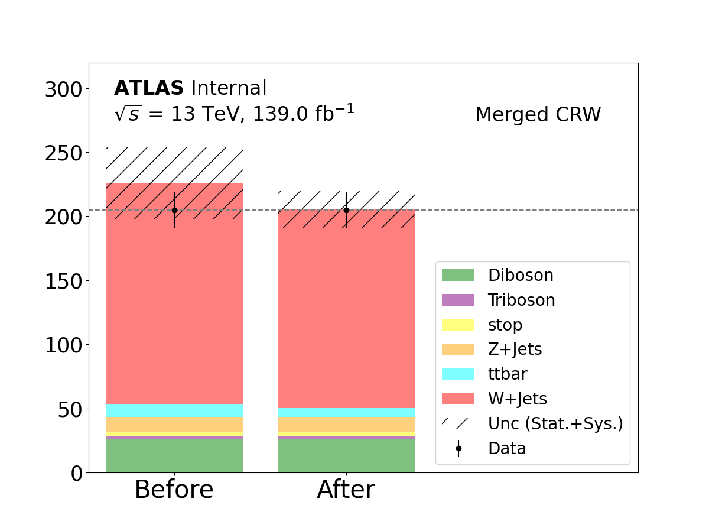
\includegraphics[width=\textwidth]{Figures/8/CRW_Merged_before_after.pdf}
    \caption{Merged CRW}\label{fig:before_after_CRW_merged}
  \end{subfigure} \hspace{1em}
  \begin{subfigure}{0.45\textwidth}
    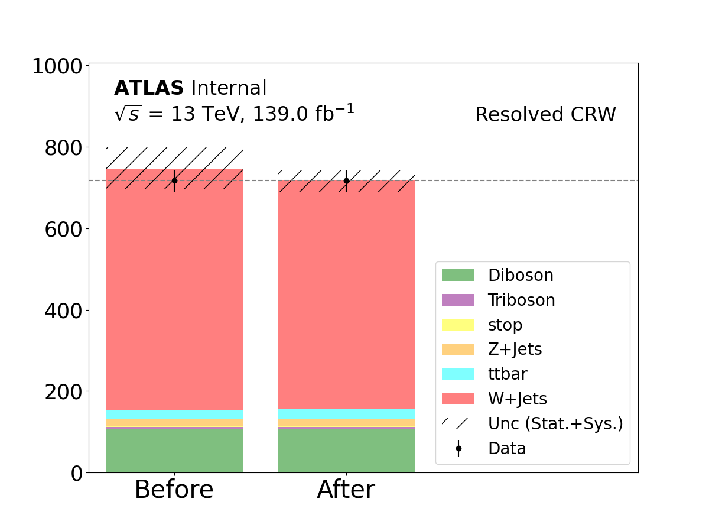
\includegraphics[width=\textwidth]{Figures/8/CRW_Resolved_before_after.pdf}
    \caption{Resolved CRW}\label{fig:before_after_CRW_resolved}
  \end{subfigure} \vspace{1em}
  \begin{subfigure}{0.45\textwidth}
    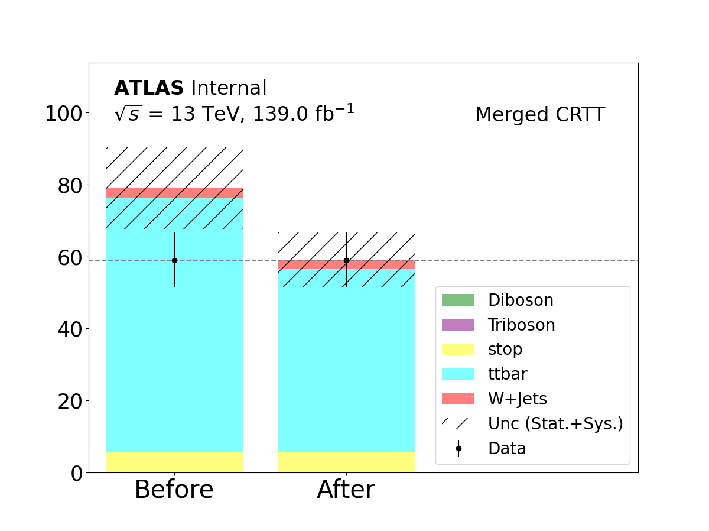
\includegraphics[width=\textwidth]{Figures/8/CRTT_Merged_before_after.pdf}
    \caption{Merged CRTT}\label{fig:before_after_CRTT_merged}
  \end{subfigure} \hspace{1em}
  \begin{subfigure}{0.45\textwidth}
    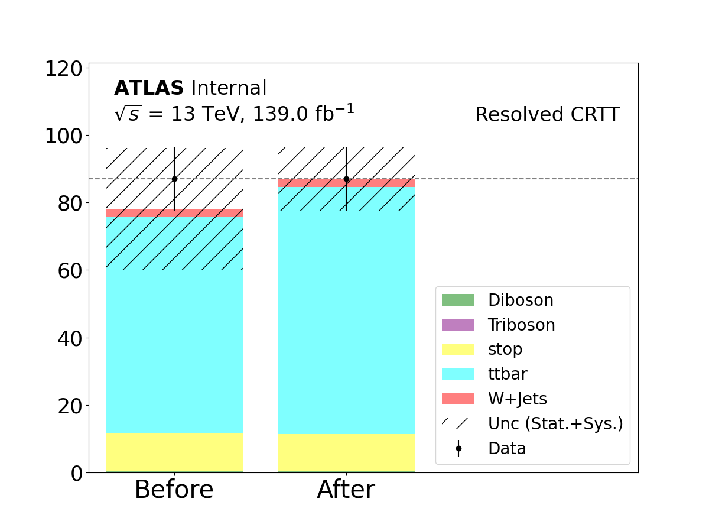
\includegraphics[width=\textwidth]{Figures/8/CRTT_Resolved_before_after.pdf}
    \caption{Resolved CRTT}\label{fig:before_after_CRTT_resolved}
  \end{subfigure} \\ \vspace{1em}
  \caption[]{Comparison between the predicted yields of SM background processes and observed yields of ATLAS collision data in the CRs, before and after the background-only fit. Hatched band shows the combined statistical and systematic uncertainty of the total yield prediction of SM background processes. Black error bars represent the Poisson uncertainty associated with the observed event count in each CR.}
  \label{fig:before_after_CRs}
\end{figure}

\subsection{Nuisance Parameter Pulls and Correlations}

Figure \ref{fig:pull_bkgonly} summarizes the post-fit shifts (a.k.a. ``pulls") of the values of all NPs included in the background-only fit, as well as their post-fit uncertainties. Both the values and uncertainties of the \(\boldsymbol{\mu}\) normalization factors, which scale the \wjets and \ttbar backgrounds separately in the merged and resolved categories, are constrained by the fit to obtain the post-fit agreement seen in Figure \ref{fig:before_after_CRs} between the total predicted yield of SM background processes and the observed yields in the ATLAS collision data. The values of all other NPs which parametrize sources of statistical and systematic uncertainty receive negligible pulls in the fit, thus indicating that good agreement with data can be obtained in all CRs just by varying the \wjets and \ttbar normalization factors. The uncertainties of the \(\gamma\)\_* parameters\footnote{See Table \ref{tab:np_naming} for a description of the scheme used to name NPs.} which parametrize the statistical uncertainty associated with the MC simulated yield predictions in each CR are reduced by the fit to data, which results in the reduction seen in Figure \ref{fig:before_after_CRs} of the uncertainty associated with the post-fit expected yield of SM background events.

\begin{figure}[h]
  \centering
  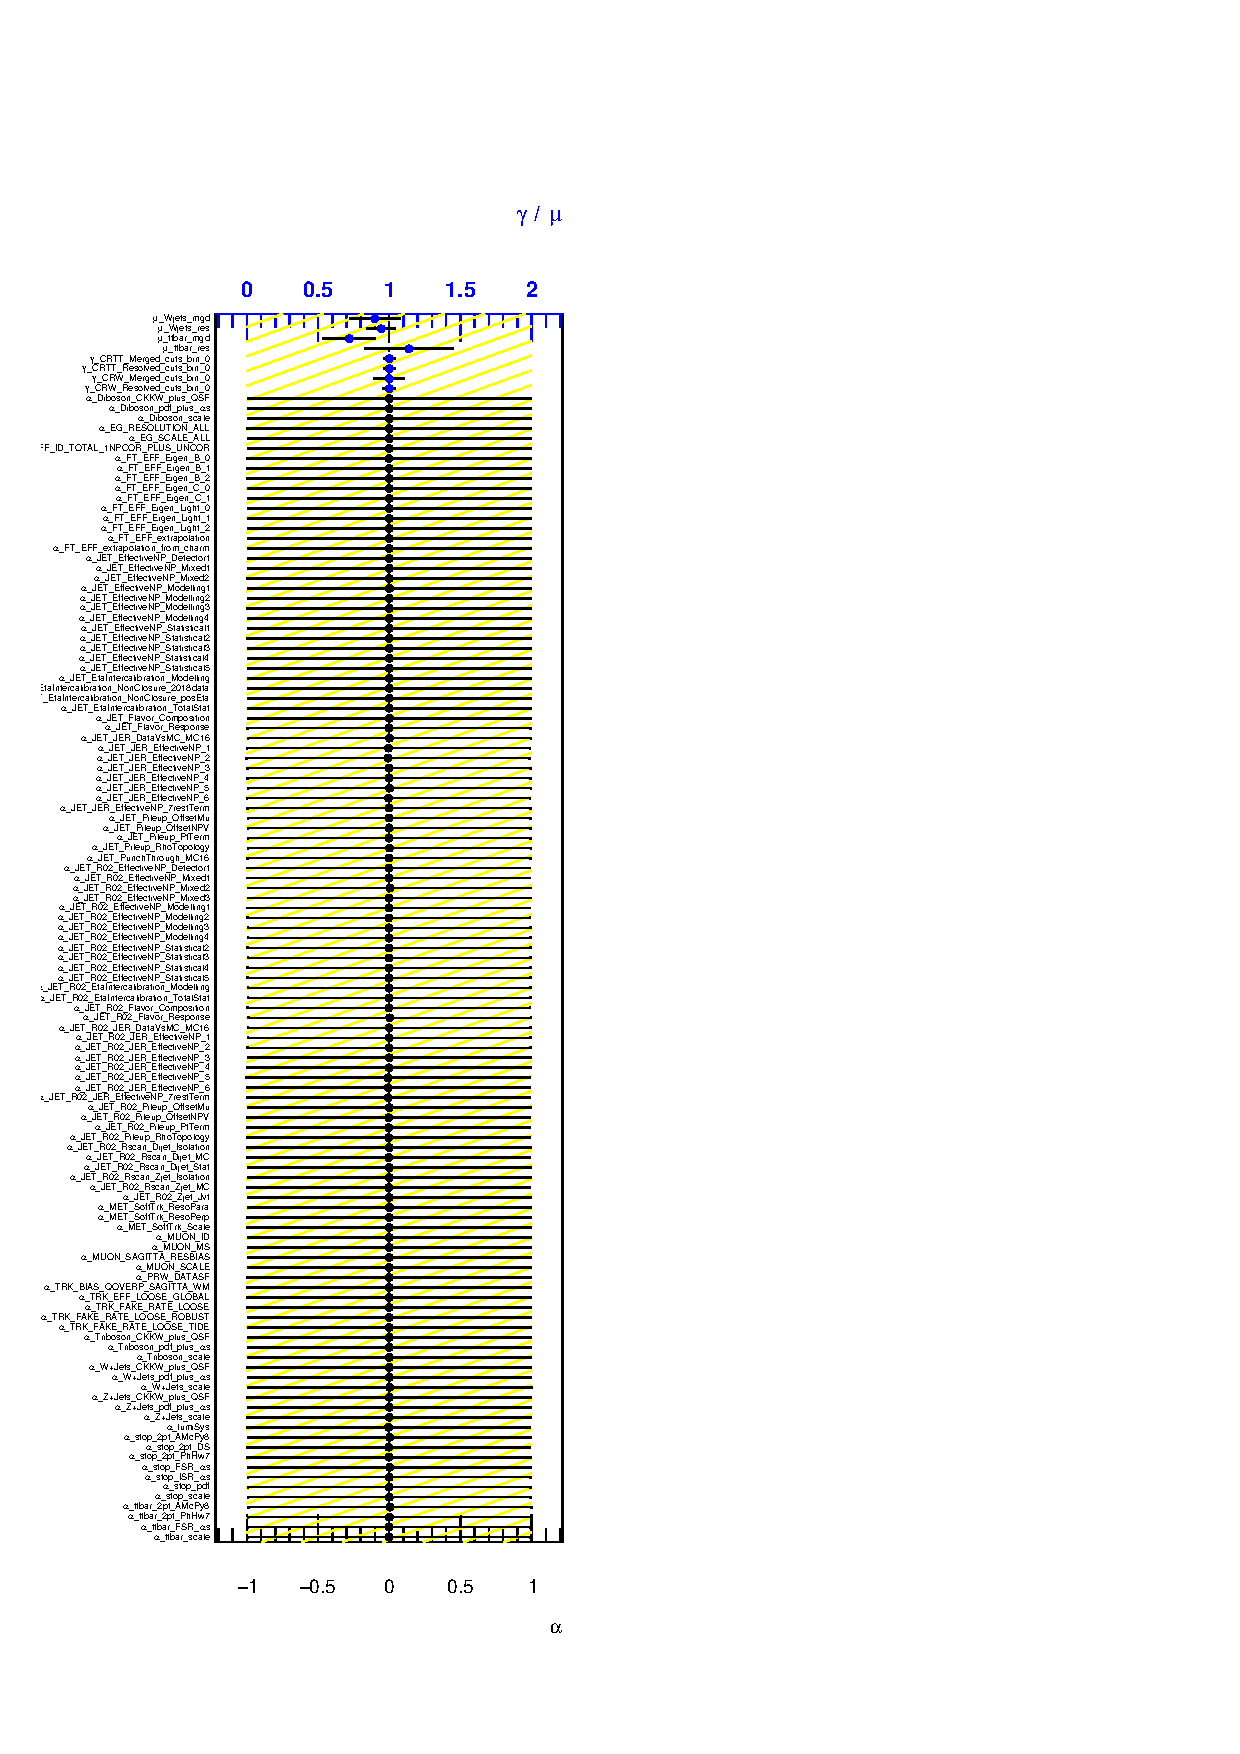
\includegraphics[width=0.55\textwidth]{Figures/8/BkgOnly/fit_parameters.pdf}
  \caption[Pull plots for background-only fit]{\footnotesize{Post-fit values and uncertainties of all NPs in the background-only fit. See Tables \ref{tab:np_naming}, \ref{tab:exp_syst_naming} and \ref{tab:theo_syst_naming} for details of the scheme used to name the NPs. Yellow hatched band shows the pre-fit uncertainty for each NP, and black horizontal error bars show the post-fit uncertainty.}}
  \label{fig:pull_bkgonly}
\end{figure}

Figure \ref{fig:corrs_bkgonly} shows the Pearson correlation coefficient \(r\) between NPs in the fit. There is some appreciable correlation (\(|r|\gtrsim0.2\)) between separate background normalization factors \(\mu\)\_*, and between normalization factors and a few of the \(\gamma\)\_* NPs - for example, \(r=-0.7\) between \(\mu\_\text{Wjets\_mgd}\) and \(\gamma\_\text{stat\_CRW\_Merged\_cuts\_bin\_0}\). However, there is in general very little cross correlation (\(r<0.01\)) between the \(\gamma\)\_* and \(\alpha\)\_* NPs which collectively parametrize all uncertainty sources in the fit due to the negligible shifts induced on these parameters by the background-only fit (see Figure \ref{fig:pull_bkgonly}).

\begin{figure}[h]
  \centering
  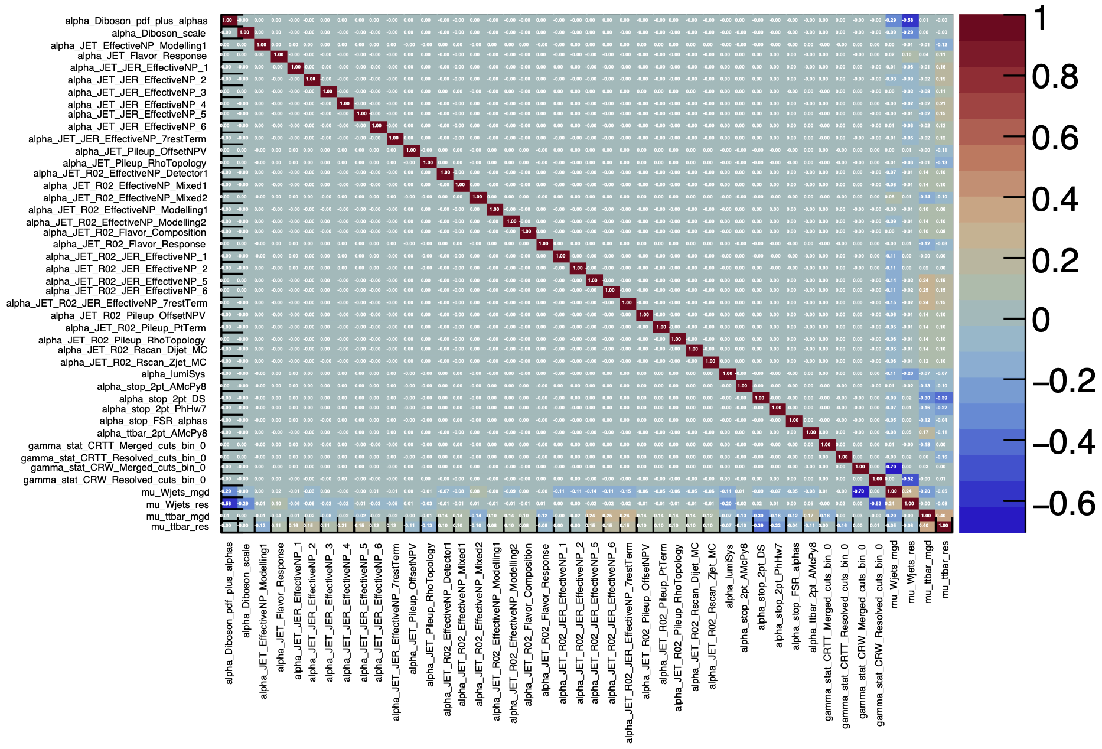
\includegraphics[width=\textwidth]{Figures/8/BkgOnly/c_corrMatrix_RooExpandedFitResult_afterFit_edited.pdf}
  \caption[Pull plots for background-only fit]{\footnotesize{Correlation matrix for all NPs considered in the background-only fit for which at least one coefficient of cross-correlation with another NP is larger than 0.1. See Tables \ref{tab:np_naming}, \ref{tab:exp_syst_naming} and \ref{tab:theo_syst_naming} for details of the scheme used to name the NPs.}}
  \label{fig:corrs_bkgonly}
\end{figure}

\section{Comparison of SM Background Expectation and Data in the Signal Region}

After performing the background-only fit in the CRs, the constraints on the background normalization factors \(\boldsymbol{\mu}\) and the other NPs \(\boldsymbol{\theta}\) summarized in Figure \ref{fig:pull_bkgonly} are extrapolated to the SR following the procedure described in Section \ref{sec:extrapolation}. Figure \ref{fig:before_after_SRs} compares the predicted yields of SM background processes in the SR - binned in \minms using the binning strategy presented in Section \ref{sec:binning_strategy} - before and after the background-only fit and extrapolation procedure. Table \ref{tab:pre_post_yields_SR} summarizes the total predicted and observed yields in the merged SRs, combined over all bins within each SR.

Both before and after the background-only fit extrapolation, Figures \ref{fig:before_SR_merged} and \ref{fig:after_SR_merged}, respectively, show an excess of observed ATLAS collision events compared with the predicted yield of SM background processes in the first three bins of the merged SR. However, the difference is within uncertainty in all three bins, and a comparison of the combined yields reported in the first row of Table \ref{tab:pre_post_yields_SR} reveals that the overall yield of ATLAS collision data in the merged SR a factor of 1.3 larger than the total post-fit uncertainty associated with the expected yield of SM background processes (a.k.a. a 1.3\(\sigma\) excess). If the distribution of measured discrepancies between the predicted yield of SM background processes and the observed yield of collision data is assumed to be reasonably approximated as Gaussian, the observed 1.3\(\sigma\) discrepancy corresponds to a two-sided p-value \cite{Stats_2003} of 0.18. If a p-value below 0.05 is taken to represent a statistically significant deviation from the null hypothesis, the observed p-value of 0.18 implies that the observed yield of ATLAS collision events in the merged SR is statistically compatible with the null hypothesis that all events observed in the SR were produced by SM background processes. 

%\begin{equation}
%\label{eq:merged_sigma}
%\frac{ \sum_{\text{bin }i\in\{\text{merged SR (S)}\}}\big[n_{S,i} - \lambda_{S,i, \text{ post-fit }}(\mu_\text{Sig}=0, \boldsymbol{\mu_i}, s_i, \boldsymbol{b_i}, \boldsymbol{\theta})\big] }{\sigma\Big(\sum_{\text{bin }i\in\{\text{merged SR (S)}\}} \lambda_{S,i}(\mu_\text{Sig}=0, \boldsymbol{\mu_i}, s_i, \boldsymbol{b_i}, \boldsymbol{\theta}) \Big)} = 1.3
%\end{equation}
%
%where \(n_{S,i}\) is the number of ATLAS collision events observed in bin \(i\) of the merged SR, \(\lambda_{S,i, \text{ post-fit }}(\mu_\text{Sig}=0, \boldsymbol{\mu_i}, s_i, \boldsymbol{b_i}, \boldsymbol{\theta})\) is the Poisson expectation defined in Eq. \ref{eq:lambda} for the total yield of MC background events in bin \(i\), assuming no signal content (\(\mu_\text{Sig}=0\)), and using values of the NPs \(\boldsymbol{\mu_i}\) and \(\boldsymbol{\theta}\) constrained in the background-only fit. \(\sigma\Big(\sum_{\text{bin }i\in\{\text{merged SR (S)}\}} \lambda_{S,i}(\mu_\text{Sig}=0, \boldsymbol{\mu_i}, s_i, \boldsymbol{b_i}, \boldsymbol{\theta}) \Big)\) is the total  uncertainty associated with the total post-fit yield expectation of SM background events in the merged SR, combined over all bins. If the ratio evaluated in Eq. \ref{eq:merged_sigma} is assumed to be sampled from a Gaussian parent distribution centred at 0 with standard deviation \(\sigma\Big(\sum_{\text{bin }i\in\{\text{merged SR (S)}\}} \lambda_{S,i}(\mu_\text{Sig}=0, \boldsymbol{\mu_i}, s_i, \boldsymbol{b_i}, \boldsymbol{\theta}) \Big)\), 

Figures \ref{fig:before_SR_resolved} and \ref{fig:after_SR_resolved} show an over-prediction of the SM background yield compared with the observed number of ATLAS collision events in all bins of the resolved SR, both before and after NP constraints from the background-only fit are extrapolated to the SRs. Comparing the observed yield of collision events from Table \ref{tab:pre_post_yields_SR} in resolved SR with the post-fit predicted yield of SM background events reveals a \(-0.8\sigma\) discrepancy. The resulting two-sided Gaussian p-value of 0.42 indicates that, as in the merged SR, the observed yields are statistically compatible with the null background-only hypothesis. 

\begin{figure}[h]
  \centering
  \begin{subfigure}{0.45\textwidth}
    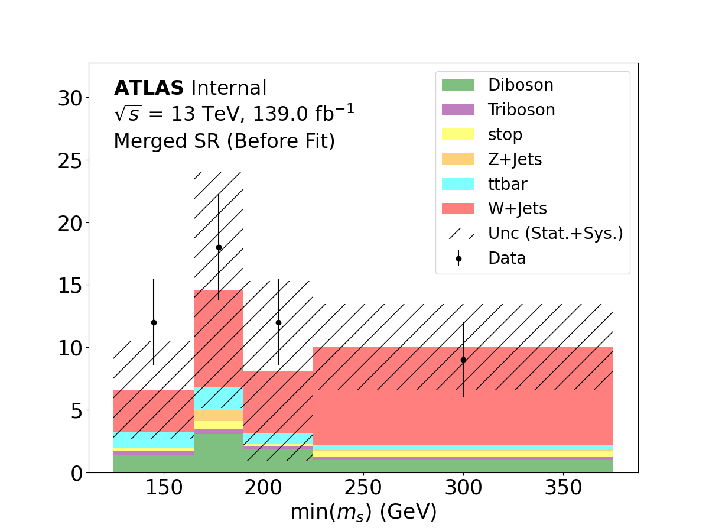
\includegraphics[width=\textwidth]{Figures/8/SR_Merged_before.pdf}
    \caption{Merged SR (Before Fit)}\label{fig:before_SR_merged}
  \end{subfigure} \hspace{1em}
  \begin{subfigure}{0.45\textwidth}
    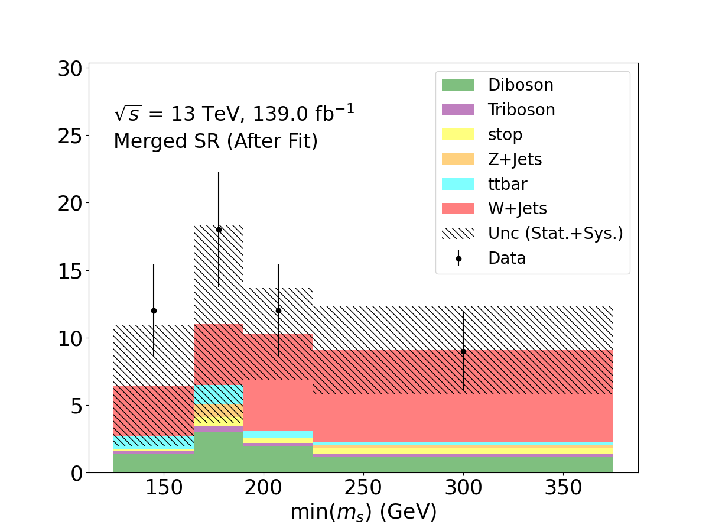
\includegraphics[width=\textwidth]{Figures/8/SR_Merged_after.pdf}
    \caption{Merged SR (After Fit)}\label{fig:after_SR_merged}
  \end{subfigure} \vspace{1em}
  \begin{subfigure}{0.45\textwidth}
    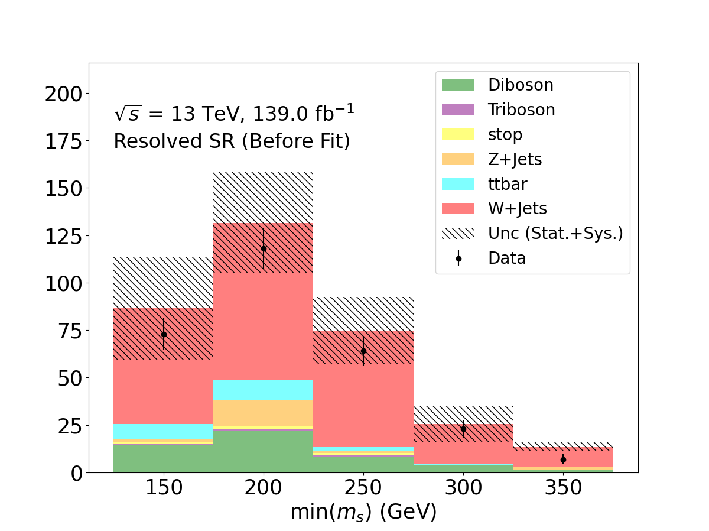
\includegraphics[width=\textwidth]{Figures/8/SR_Resolved_before.pdf}
    \caption{Resolved SR (Before Fit)}\label{fig:before_SR_resolved}
  \end{subfigure} \hspace{1em}
  \begin{subfigure}{0.45\textwidth}
    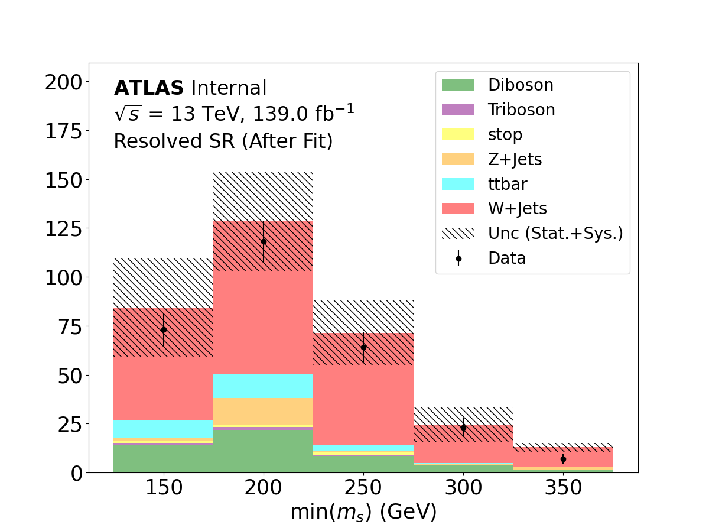
\includegraphics[width=\textwidth]{Figures/8/SR_Resolved_after.pdf}
    \caption{Resolved SR (After Fit)}\label{fig:after_SR_resolved}
  \end{subfigure} \\ \vspace{1em}
  \caption[]{Comparison between predicted yields of SM background processes and observed yields in the SRs, before (left) and after (right) the background-only fit and extrapolation to the SR. Yields are binned in \minms using the binning strategy presented in Section \ref{sec:binning_strategy}.}
  \label{fig:before_after_SRs}
\end{figure}

\begin{table}
\centering
\caption{Comparison of the total observed yields of events in the SRs with the predicted yield of SM background processes, either before (pre-fit) or after (post-fit) extrapolation of constraints from the background-only fit in the CRs.}
\label{tab:pre_post_yields_SR}
\begin{tabular}{l l l l}
\toprule
\textbf{Region} & \textbf{Observed Yield} & \textbf{SM Bkg Prediction} & \textbf{SM Bkg Prediction} \\
 & & \textbf{(Pre-fit)} & \textbf{(Post-fit)} \\
\midrule
\midrule
Merged SR & 51 & $39.3 \pm 13$ & $35.7 \pm 12$ \\
\midrule
Resolved SR & 285 & $333.3\pm 69$ & $323.4 \pm 50$ \\
\bottomrule
\end{tabular}
\end{table}

\section{Exclusion of the Dark Higgs Signal Model}

Given the absence of any statistically significant discrepancy between the observed yields of ATLAS collision events in the SRs and the predicted yields of events from SM background processes, the exclusion hypothesis test presented in Section \ref{sec:hypo_test} is used to determine the range of \ms and \mZp for which the DH signal model can be confidently excluded by the search for the fixed choices of the DM mass \(\mchi\), mixing angle \(\sin\theta\) and coupling choices \(g_q\) and \(\gchi\) in the DH model used for the search\footnote{See Sections \ref{sec:dh_model_free_parameters} and \ref{sec:dh_searches} for a presentation and discussion of the choices for the \mchi, \(\sin\theta\) and coupling parameters in the DH model.}:

\begin{itemize}
\item \(\mchi=200~\GeV\)
\item \(g_q=0.25\)
\item \(g_\chi=1\)
\item \(\sin\theta=0.01\)
\end{itemize}

\subsection{Signal+Background Fit}

Figures \ref{fig:before_after_SRs_MonoSlep_monoSWWsemilep_zp1000_dm200_dh160}, \ref{fig:before_after_SRs_MonoSlep_monoSWWsemilep_zp2100_dm200_dh210} and \ref{fig:before_after_SRs_MonoSlep_monoSWWsemilep_zp2900_dm200_dh310} compare the observed yield of ATLAS collision events in the SRs, binned in \minms, with the predicted yields for the SM background and DH signal processes at the three sample combinations of \ms and \mZp in the signal model. The sample \ms and \mZp combinations, listed below, are chosen to cover the range of production cross sections for the DH model considered in the search:

\begin{itemize}
\item \((\ms, \mZp) = (160, 1000)~\GeV\) (cross section: 93.3 fb\(^{-1}\))
\item \((\ms, \mZp) = (210, 2100)~\GeV\) (cross section: 3.9 fb\(^{-1}\))
\item \((\ms, \mZp) = (310, 2900)~\GeV\) (cross section: 0.31 fb\(^{-1}\))
\end{itemize}

As shown in Figure \ref{fig:before_after_SRs_MonoSlep_monoSWWsemilep_zp1000_dm200_dh160}, the DH signal model at \((\ms, \mZp) = (160, 1000)~\GeV\) with a cross section of 93.3 fb\({^{-1}}\) has a sufficiently large production rate that the signal+background fit constrains the signal strength parameter to \(\mu_\text{Sig}=0.09\pm0.08\). Therefore, the signal+background hypothesis (\(\mu_\text{Sig}=1\)) is excluded with a high degree of confidence.

Figure \ref{fig:before_after_SRs_MonoSlep_monoSWWsemilep_zp2100_dm200_dh210} shows the results of the signal+background fit for \((\ms, \mZp) = (210, 2100)~\GeV\) in the signal model, with an intermediate cross section of 3.9 fb\(^{-1}\). The predicted yield of the signal process is comparable in the first three bins of the merged SR to the discrepancy between the observed yield of data and the predicted yield of SM background processes, which results in a fitted signal strength close to 1 (\(\mu_\text{Sig}=0.88\)). However, since the predicted yield of the signal and background processes are still consistent with the background-only prediction, there is a large (nearly 100\%) uncertainty associated with the fitted signal strength. As a result, the fit can neither support nor confidently exclude the signal+background hypothesis at this mass point. 

Further reduced exclusion power is observed for the fit shown in Figure \ref{fig:after_SR_merged_MonoSlep_monoSWWsemilep_zp2900_dm200_dh310} which considers the signal model at the mass combination \((\ms, \mZp) = (310, 2900)~\GeV\) with the lowest cross section of the three combinations considered. The signal yields are so small compared with the uncertainty of the total yield prediction that the fitted signal strength could range from \(-3.82\) to \(5.06\) within its post-fit uncertainty. As a result, the search can neither meaningfully support nor exclude the DH signal model at this mass point.

\begin{figure}[h]
  \centering
  \begin{subfigure}{0.45\textwidth}
    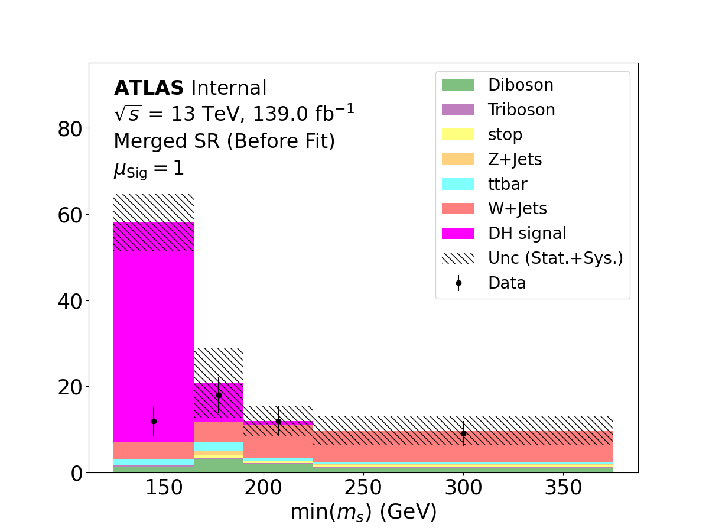
\includegraphics[width=\textwidth]{Figures/8/MonoSlep_monoSWWsemilep_zp1000_dm200_dh160/SR_Merged_before.pdf}
    \caption{Merged SR (Before Fit)}\label{fig:before_SR_merged_MonoSlep_monoSWWsemilep_zp1000_dm200_dh160}
  \end{subfigure} \hspace{1em}
  \begin{subfigure}{0.45\textwidth}
    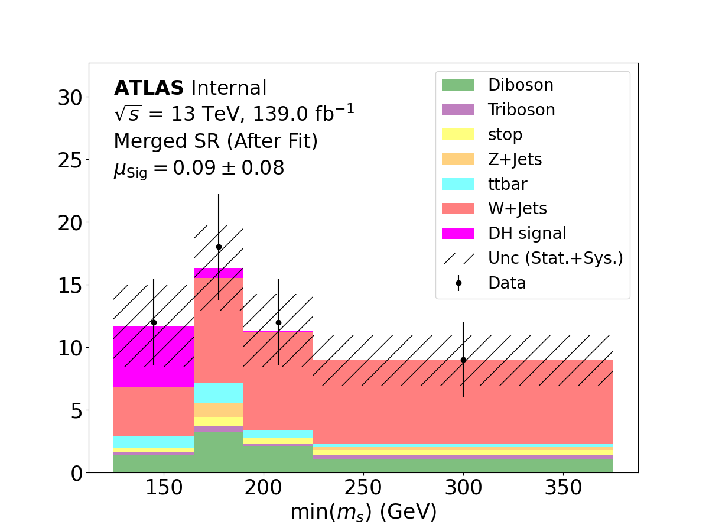
\includegraphics[width=\textwidth]{Figures/8/MonoSlep_monoSWWsemilep_zp1000_dm200_dh160/SR_Merged_after.pdf}
    \caption{Merged SR (After Fit)}\label{fig:after_SR_resolved_MonoSlep_monoSWWsemilep_zp1000_dm200_dh160}
  \end{subfigure} \vspace{1em}
  \begin{subfigure}{0.45\textwidth}
    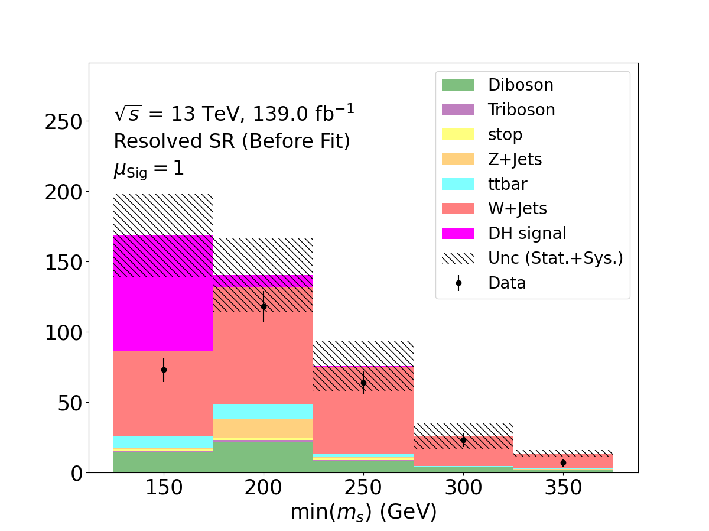
\includegraphics[width=\textwidth]{Figures/8/MonoSlep_monoSWWsemilep_zp1000_dm200_dh160/SR_Resolved_before.pdf}
    \caption{Resolved SR (Before Fit)}\label{fig:before_SR_merged_MonoSlep_monoSWWsemilep_zp1000_dm200_dh160}
  \end{subfigure} \hspace{1em}
  \begin{subfigure}{0.45\textwidth}
    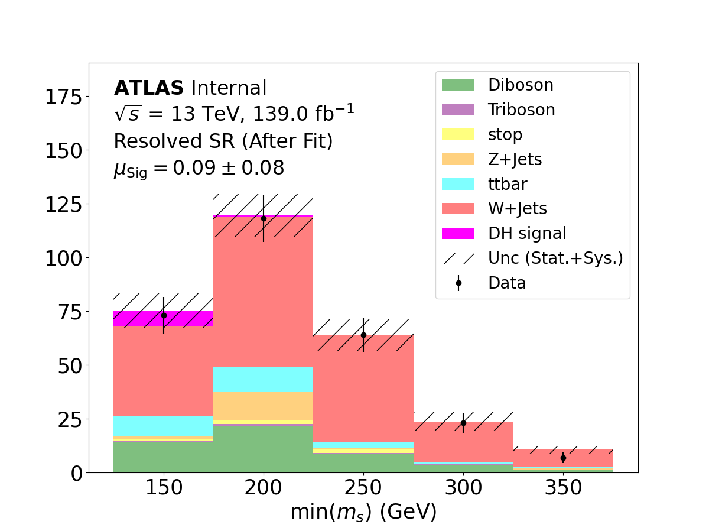
\includegraphics[width=\textwidth]{Figures/8/MonoSlep_monoSWWsemilep_zp1000_dm200_dh160/SR_Resolved_after.pdf}
    \caption{Resolved SR (After Fit)}\label{fig:after_SR_merged_MonoSlep_monoSWWsemilep_zp1000_dm200_dh160}
  \end{subfigure} \\ \vspace{1em}
  \caption[]{Comparison between predicted yields of SM background processes, the DH signal process at \((\ms, \mZp) = (160, 1000)~\GeV\) and observed yields in the SRs. Yields are shown before (left) and after (right) the signal+background fit. The pre-and post-fit values of the signal strength \(\mu_\text{Sig}\) are also reported. Yields are binned in \minms using the binning strategy presented in Section \ref{sec:binning_strategy}.}
  \label{fig:before_after_SRs_MonoSlep_monoSWWsemilep_zp1000_dm200_dh160}
\end{figure}

\begin{figure}[h]
  \centering
  \begin{subfigure}{0.45\textwidth}
    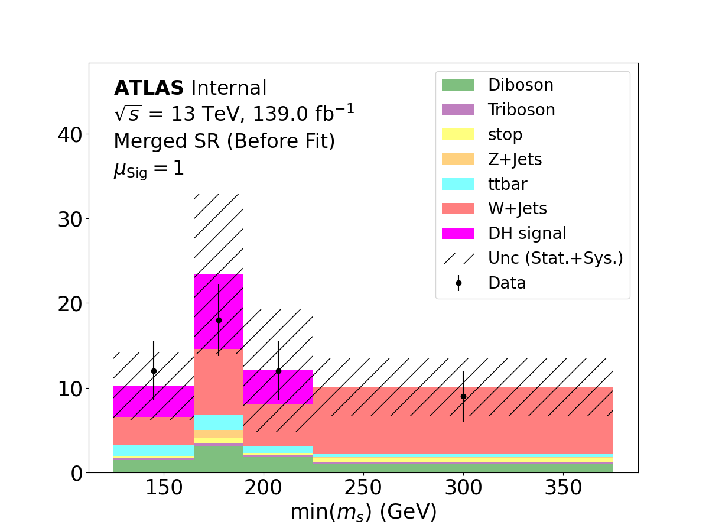
\includegraphics[width=\textwidth]{Figures/8/MonoSlep_monoSWWsemilep_zp2100_dm200_dh210/SR_Merged_before.pdf}
    \caption{Merged SR (Before Fit)}\label{fig:before_SR_merged_MonoSlep_monoSWWsemilep_zp2100_dm200_dh210}
  \end{subfigure} \hspace{1em}
  \begin{subfigure}{0.45\textwidth}
    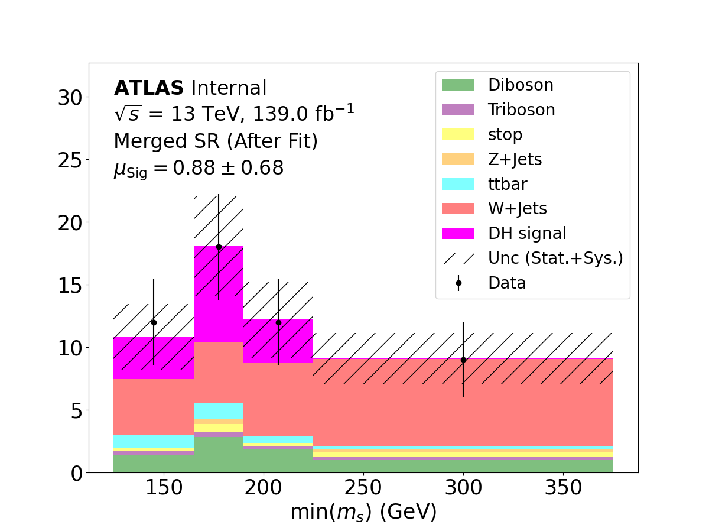
\includegraphics[width=\textwidth]{Figures/8/MonoSlep_monoSWWsemilep_zp2100_dm200_dh210/SR_Merged_after.pdf}
    \caption{Merged SR (After Fit)}\label{fig:after_SR_resolved_MonoSlep_monoSWWsemilep_zp2100_dm200_dh210}
  \end{subfigure} \vspace{1em}
  \begin{subfigure}{0.45\textwidth}
    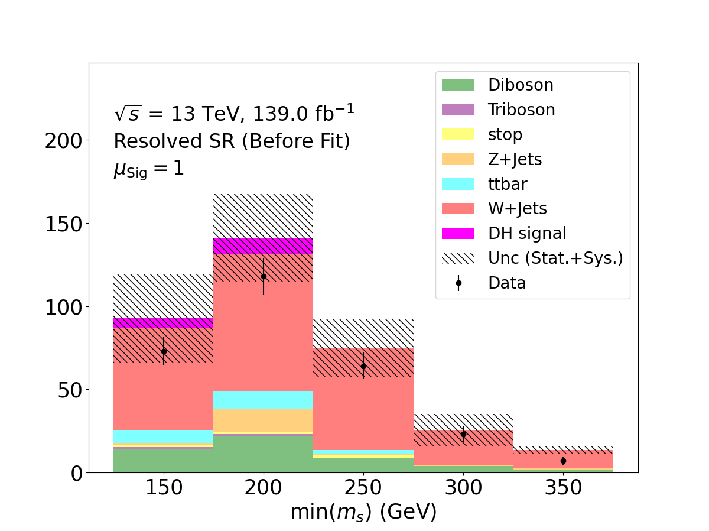
\includegraphics[width=\textwidth]{Figures/8/MonoSlep_monoSWWsemilep_zp2100_dm200_dh210/SR_Resolved_before.pdf}
    \caption{Resolved SR (Before Fit)}\label{fig:before_SR_merged_MonoSlep_monoSWWsemilep_zp2100_dm200_dh210}
  \end{subfigure} \hspace{1em}
  \begin{subfigure}{0.45\textwidth}
    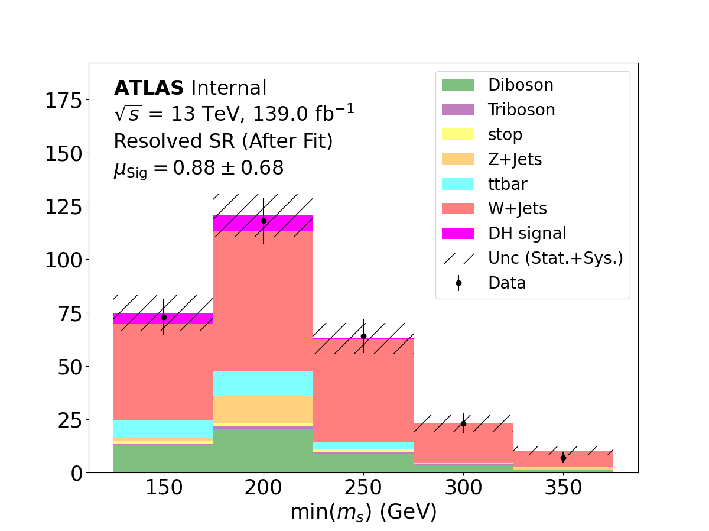
\includegraphics[width=\textwidth]{Figures/8/MonoSlep_monoSWWsemilep_zp2100_dm200_dh210/SR_Resolved_after.pdf}
    \caption{Resolved SR (After Fit)}\label{fig:after_SR_merged_MonoSlep_monoSWWsemilep_zp2100_dm200_dh210}
  \end{subfigure} \\ \vspace{1em}
  \caption[]{Comparison between predicted yields of SM background processes, the DH signal process at \((\ms, \mZp) = (210, 2100)~\GeV\) and observed yields in the SRs. Yields are shown before (left) and after (right) the signal+background fit. The pre-and post-fit values of the signal strength \(\mu_\text{Sig}\) are also reported. Yields are binned in \minms using the binning strategy presented in Section \ref{sec:binning_strategy}.}
  \label{fig:before_after_SRs_MonoSlep_monoSWWsemilep_zp2100_dm200_dh210}
\end{figure}

\begin{figure}[h]
  \centering
  \begin{subfigure}{0.45\textwidth}
    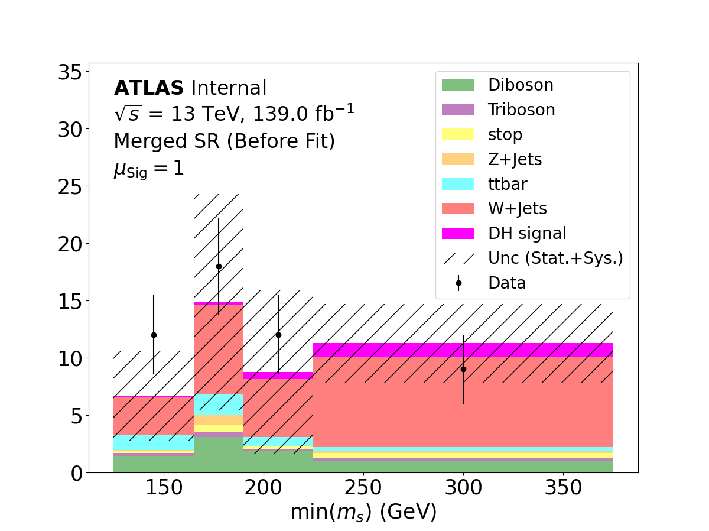
\includegraphics[width=\textwidth]{Figures/8/MonoSlep_monoSWWsemilep_zp2900_dm200_dh310/SR_Merged_before.pdf}
    \caption{Merged SR (Before Fit)}\label{fig:before_SR_merged_MonoSlep_monoSWWsemilep_zp2900_dm200_dh310}
  \end{subfigure} \hspace{1em}
  \begin{subfigure}{0.45\textwidth}
    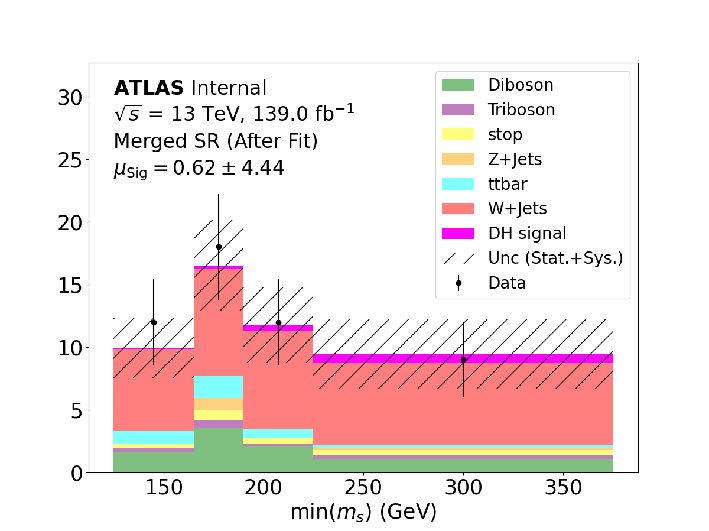
\includegraphics[width=\textwidth]{Figures/8/MonoSlep_monoSWWsemilep_zp2900_dm200_dh310/SR_Merged_after.pdf}
    \caption{Merged SR (After Fit)}\label{fig:after_SR_resolved_MonoSlep_monoSWWsemilep_zp2900_dm200_dh310}
  \end{subfigure} \vspace{1em}
  \begin{subfigure}{0.45\textwidth}
    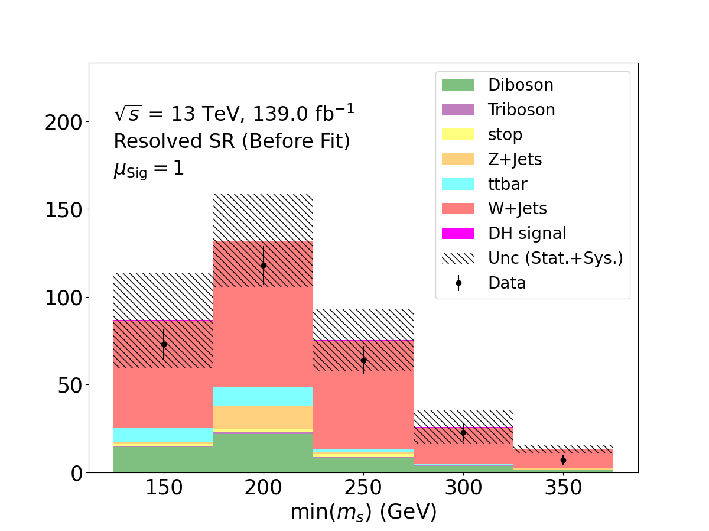
\includegraphics[width=\textwidth]{Figures/8/MonoSlep_monoSWWsemilep_zp2900_dm200_dh310/SR_Resolved_before.pdf}
    \caption{Resolved SR (Before Fit)}\label{fig:before_SR_merged_MonoSlep_monoSWWsemilep_zp2900_dm200_dh310}
  \end{subfigure} \hspace{1em}
  \begin{subfigure}{0.45\textwidth}
    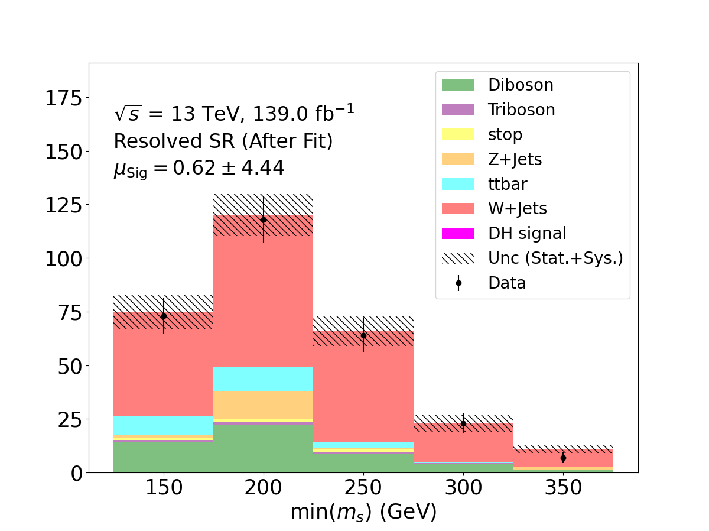
\includegraphics[width=\textwidth]{Figures/8/MonoSlep_monoSWWsemilep_zp2900_dm200_dh310/SR_Resolved_after.pdf}
    \caption{Resolved SR (After Fit)}\label{fig:after_SR_merged_MonoSlep_monoSWWsemilep_zp2900_dm200_dh310}
  \end{subfigure} \\ \vspace{1em}
  \caption[]{Comparison between predicted yields of SM background processes, the DH signal process at \((\ms, \mZp) = (310, 2900)~\GeV\) and observed yields in the SRs. Yields are shown before (left) and after (right) the signal+background fit. The pre-and post-fit values of the signal strength \(\mu_\text{Sig}\) are also reported. Yields are binned in \minms using the binning strategy presented in Section \ref{sec:binning_strategy}.}
  \label{fig:before_after_SRs_MonoSlep_monoSWWsemilep_zp2900_dm200_dh310}
\end{figure}

Figure \ref{fig:fitted_mu_Sig} summarizes the post-fit value and uncertainty of the signal strength parameter \(\mu_\text{Sig}\) for the signal+background fit performed with the DH signal model at all \ms and \mZp considered in the search. The fitted value and uncertainty vary depending on the production cross section and the shape of the signal distribution with respect to \minms. The size of the uncertainty for a given \ms and \mZp combination reflects the exclusion power of the search at the given mass combination, where a larger uncertainty generally implies less exclusion power. In general, the fitted values of \(\mu_\text{Sig}\) are consistent with 0 within 1.5\(\sigma\), in agreement with the null background-only hypothesis.

\begin{figure}[h]
  \centering
  \begin{subfigure}{0.49\textwidth}
    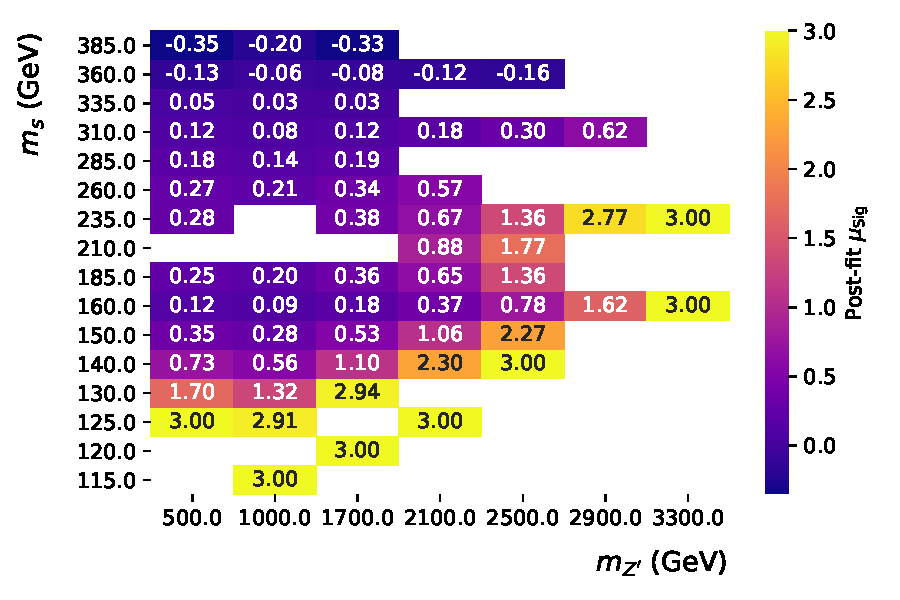
\includegraphics[width=\textwidth]{Figures/8/mu_sigs.pdf}
    \caption{Post-fit \(\mu_\text{Sig}\)}\label{fig:fitted_mu_Sig}
  \end{subfigure} 
  \begin{subfigure}{0.49\textwidth}
    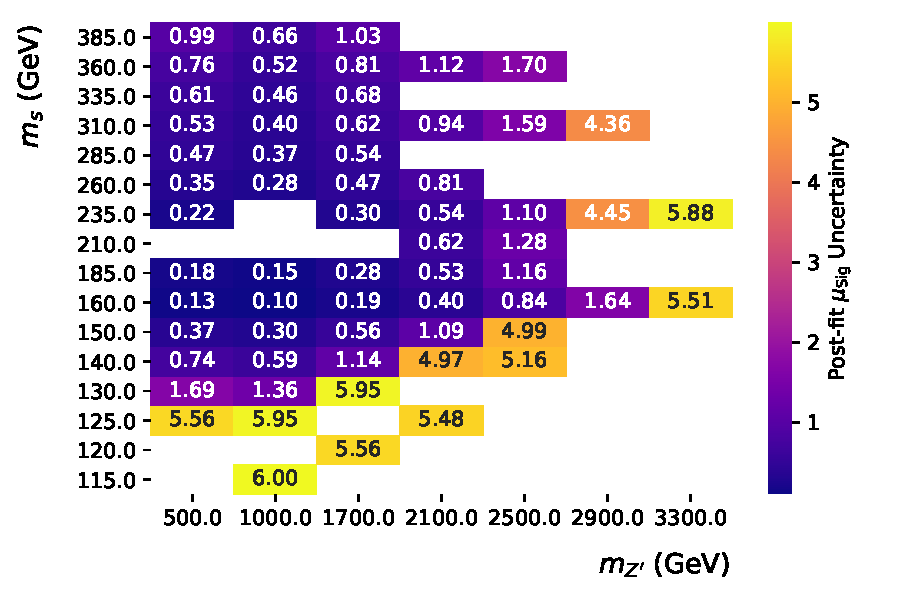
\includegraphics[width=\textwidth]{Figures/8/mu_sig_unc.pdf}
    \caption{Post-fit \(\mu_\text{Sig}\) uncertainty}\label{fig:fitted_mu_Sig_unc}
  \end{subfigure} 
  \caption[]{Post-fit value (left) and uncertainty (right) of the signal strength parameter \(\mu_\text{Sig}\) in the signal+background fit (\(\mu_\text{Sig}\) left floating) for each \ms and \mZp in the DH signal model.}
  \label{fig:fitted_mu_Sig}
\end{figure}

\subsubsection{Nuisance Parameter Pulls and Correlations}
\label{sec:np_pulls_sig_plus_bkg}

Figure \ref{fig:pull_sigPlusBkg} summarizes the pulls and uncertainties of all NPs included in the signal+background fit using the DH signal model at the sample mass point \((\ms, \mZp) = (210, 2100)~\GeV\). In contrast with the background-only fit, the pulls of some \(\gamma\)\_* and \(\alpha\)\_* NPs which constrain the statistical and systematic uncertainties associated with MC simulated yields can be appreciably shifted (i.e. pulled) relative to their pre-fit values. This is due to differences in the shapes of \minms distributions in the SRs between the observed ATLAS collision data and the predicted yields of the SM background and signal processes, which cannot be corrected by varying the \(\mu\)\_* normalization parameters alone. Particularly large pulls are seen for the NPs \(\alpha\)\_JET\_JER\_* and \(\alpha\)\_JET\_R02\_JER\_* which parametrize the systematic jet energy resolution (JER) uncertainties associated with the \(R=0.4\)\footnote{See Section \ref{sec:atk4_jets} for a description of the \(R=0.4\) jets, and Section \ref{sec:resolved_w_cand} for a description of the method used to reconstruct the \(W\) boson candidate in the resolved category.} and \(R=0.2\)\footnote{See Section \ref{sec:TAR_algo} for a description of the algorithm used to construct TAR jets using input \(R=0.2\) jets.}  jets, respectively (see Tables \ref{tab:exp_syst_naming} and \ref{tab:theo_syst_naming} for descriptions of individual NPs used to parametrize systematic uncertainties). As shown in Figures \ref{fig:exp_syst_shifts_bkg} and \ref{fig:exp_syst_shifts_sig}, the JER systematic uncertainties induce the largest yield shifts in the SRs relative to other systematic sources. Therefore, it is reasonable to expect that these NPs would in general receive relatively strong pulls in the signal+background fit to help correct for the observed differences between expected and observed event yields in the SRs. 

\begin{figure}[h]
  \centering
  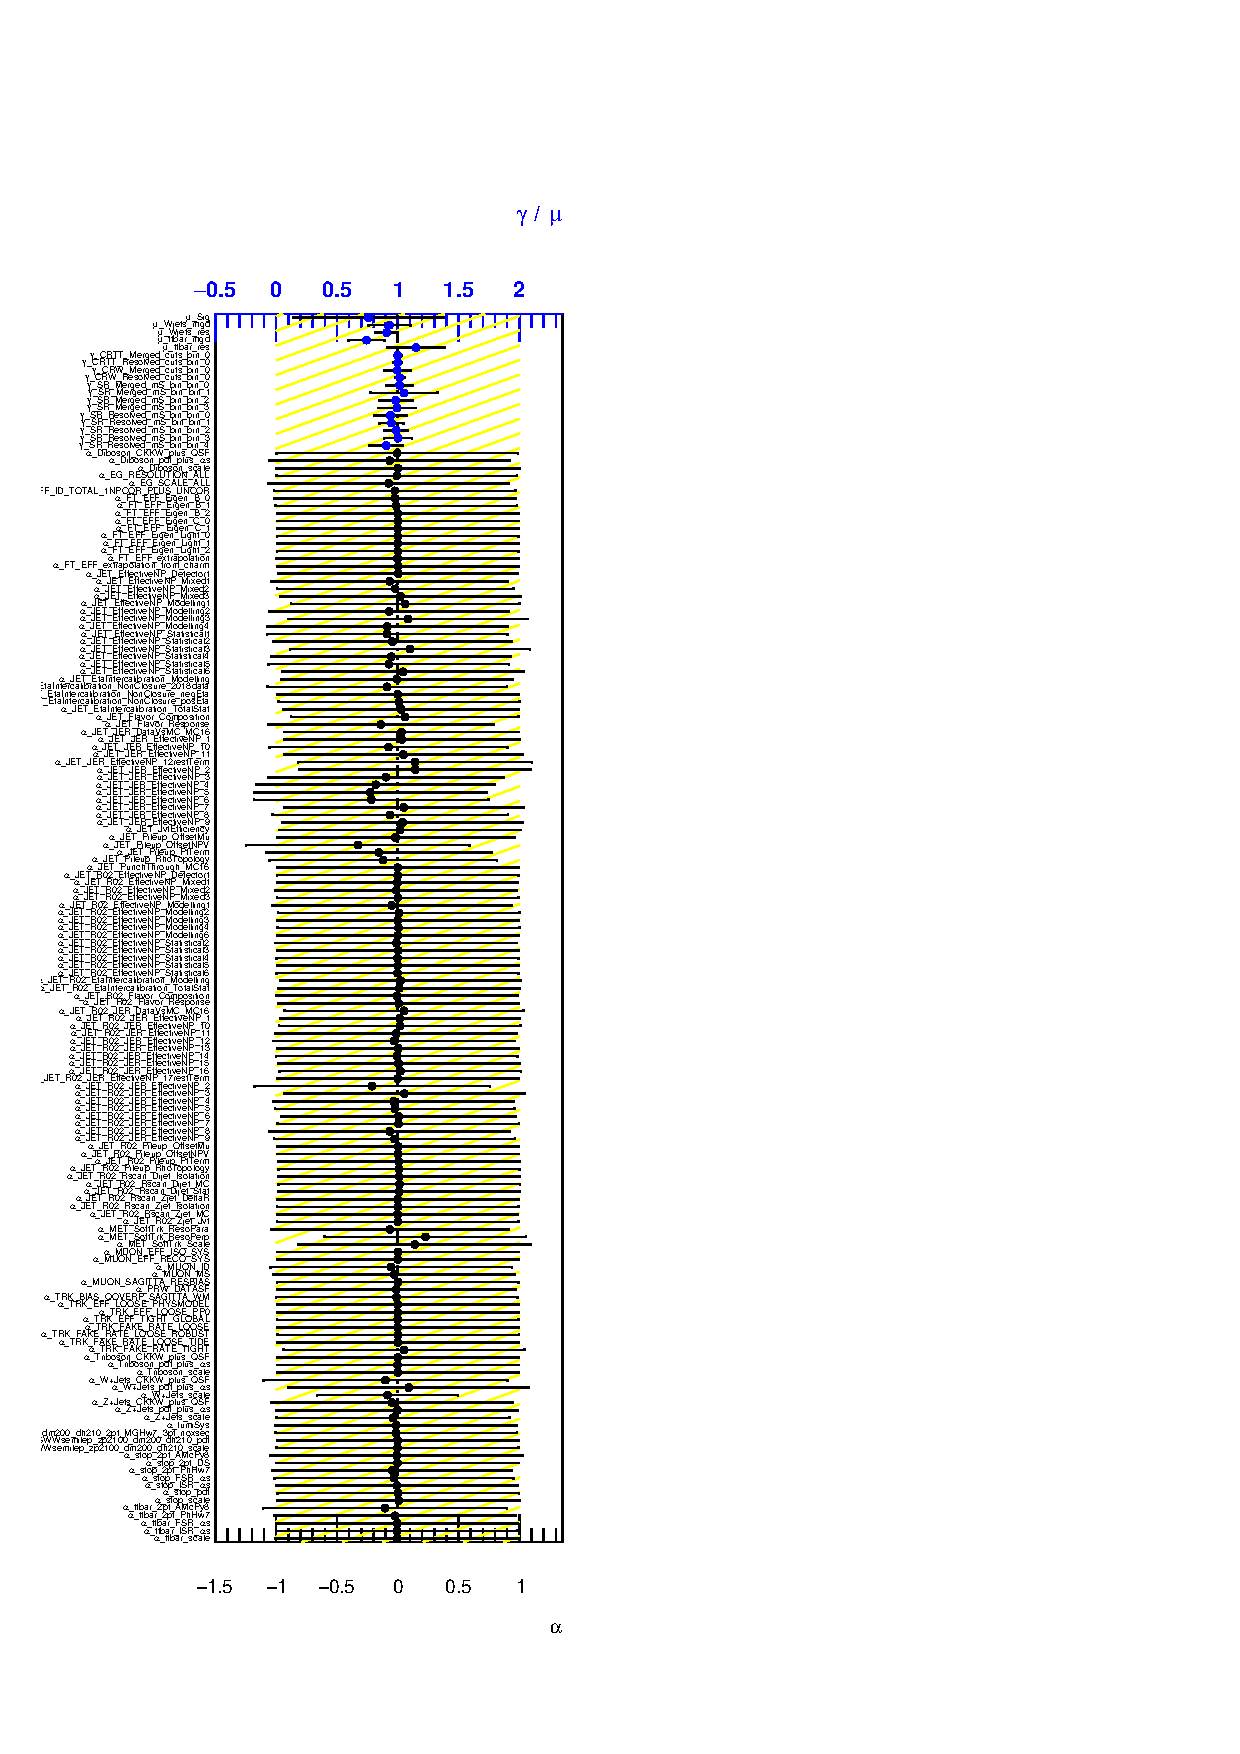
\includegraphics[width=0.5\textwidth]{Figures/8/MonoSlep_monoSWWsemilep_zp2100_dm200_dh210/fit_parameters.pdf}
  \caption[Pull plots for blinded SRs]{\footnotesize{Post-fit values of all NPs in the signal+background fit using the DH signal model at \((\ms, \mZp) = (210, 2100)~\GeV\). See Tables \ref{tab:np_naming}, \ref{tab:exp_syst_naming} and \ref{tab:theo_syst_naming} for details of the scheme used to name the NPs. Yellow hatched band shows the pre-fit uncertainty for each NP, and black horizontal error bars show the post-fit uncertainty.}}
  \label{fig:pull_sigPlusBkg}
\end{figure}

Figure \ref{fig:corrs_sigPlusBkg} shows the Pearson correlation coefficient \(r\) between NPs in the signal+background fit for the sample mass point \((\ms, \mZp) = (210, 2100)~\GeV\) in the DH signal model. As with the background-only fit, there is appreciable correlation (\(|r|\gtrsim0.2\)) between separate background normalization factors \(\mu\)\_*, and between normalization factors and several of the \(\gamma\)\_* NPs which parametrize the statistical uncertainties associated with MC simulated yield predictions. In contrast to the background-only fit, some of the \(\alpha\)\_* parameters also have non-negligible correlations (\(|r|\) up to \(\sim0.3\)) with one another and with \(\gamma\)\_* and \(\mu\)\_* NPs. The introduction of correlations involving \(\alpha\)\_* NPs in the signal+background fit compared with the background-only fit is attributed to the non-negligible post-fit shifts of these NPs observed in Figure \ref{fig:pull_sigPlusBkg} for the signal+background fit.

\begin{figure}[h]
  \centering
  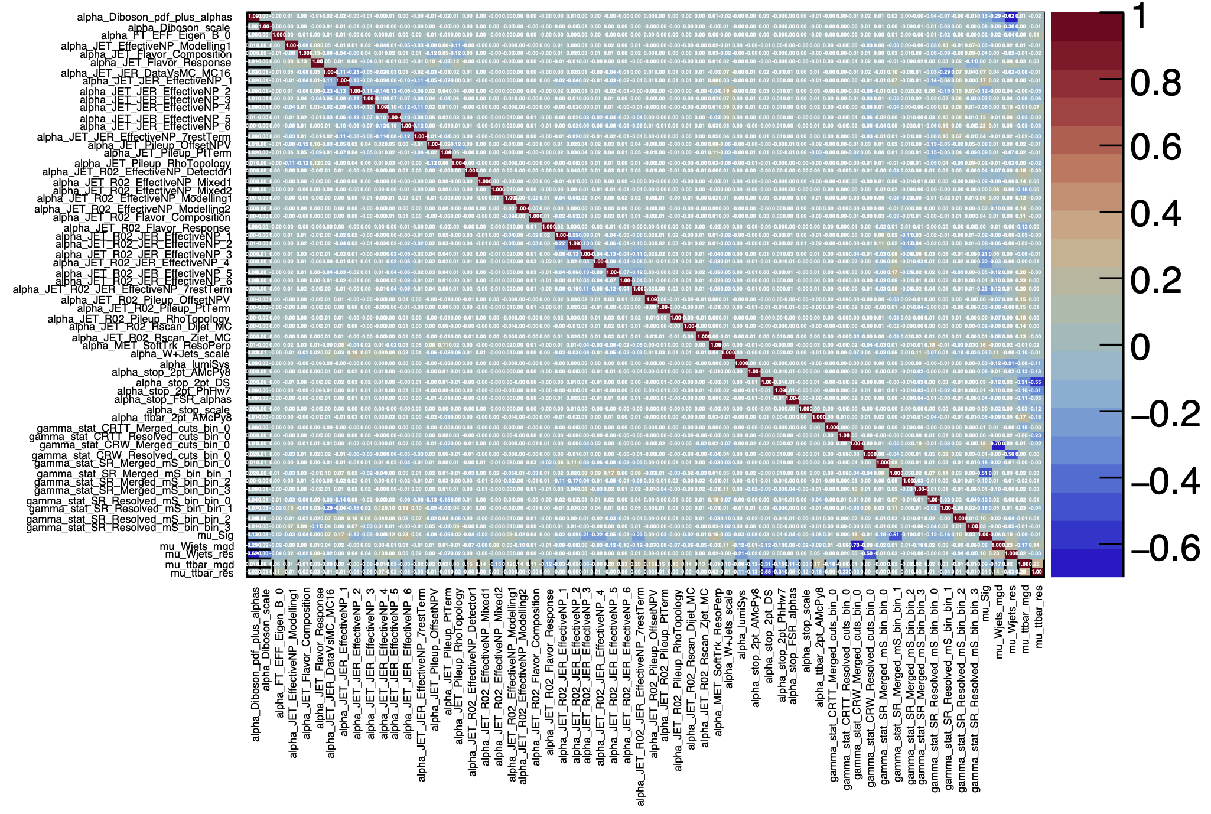
\includegraphics[width=\textwidth]{Figures/8/MonoSlep_monoSWWsemilep_zp2100_dm200_dh210/c_corrMatrix_RooExpandedFitResult_afterFit_edited.pdf}
  \caption[Pull plots for blinded SRs]{\footnotesize{Correlation matrix for all NPs considered in the signal+background fit at a sample signal point of \((\ms, \mZp) = (210, 2100)~\GeV\), for which at least one coefficient of cross-correlation with another NP is larger than 0.1. See Tables \ref{tab:np_naming}, \ref{tab:exp_syst_naming} and \ref{tab:theo_syst_naming} for details of the scheme used to name the NPs.}}
  \label{fig:corrs_sigPlusBkg}
\end{figure}

\subsubsection{Ranking of Systematic Uncertainties}

Figure \ref{fig:ranking_ms210} shows the pre- and post-fit values and impacts of NPs in the signal+background fit on the fitted signal strength \(\mu_\text{Sig}\). The 30 leading NPs are ranked from top to bottom in order of the size of their impact. The pre- and post-fit impact of a given NP \(\theta\) is measured as follows:

\begin{itemize}
    \item \textbf{Pre-fit impact:} Shift the value of \(\theta\) to the upper bound \(\theta_0+\Delta\theta\) of its pre-fit uncertainty. Perform the signal+background fit with \(\theta\) fixed to this upper value, and all other NPs left floating. Repeat with the value of \(\theta\) fixed to the lower bound \(\theta_0+\Delta\theta\) of its pre-fit uncertainty. The resulting shifts \(\Delta_\text{up/down}{\reallywidehat{\mu_\text{Sig}}}\) of the best-fit \(\mu_\text{Sig}\) are shown as unfilled white boxes with black borders in Figure \ref{fig:ranking_ms210}.
    \item \textbf{Post-fit impact:} As above, but with the value of \(\theta\) shifted instead to the upper and lower bounds of its post-fit uncertainty. The resulting shifts \(\Delta_\text{up/down}{\reallywidehat{\mu_\text{Sig}}}\) are shown as filled boxes, where the colour of the box indicates whether \(\mu_\text{Sig}\) is correlated (blue) or anti-correlated (green) with the value of the NP.
\end{itemize}

The highest-ranked NPs are associated with systematic JER uncertainties, which also receive some of the largest pulls in the fit (see Figure \ref{fig:pull_sigPlusBkg} and related discussion in Section \ref{sec:np_pulls_sig_plus_bkg}). Following in rank are some of the statistical \(\gamma\)\_* NPs. 

\begin{figure}[h]
  \centering
  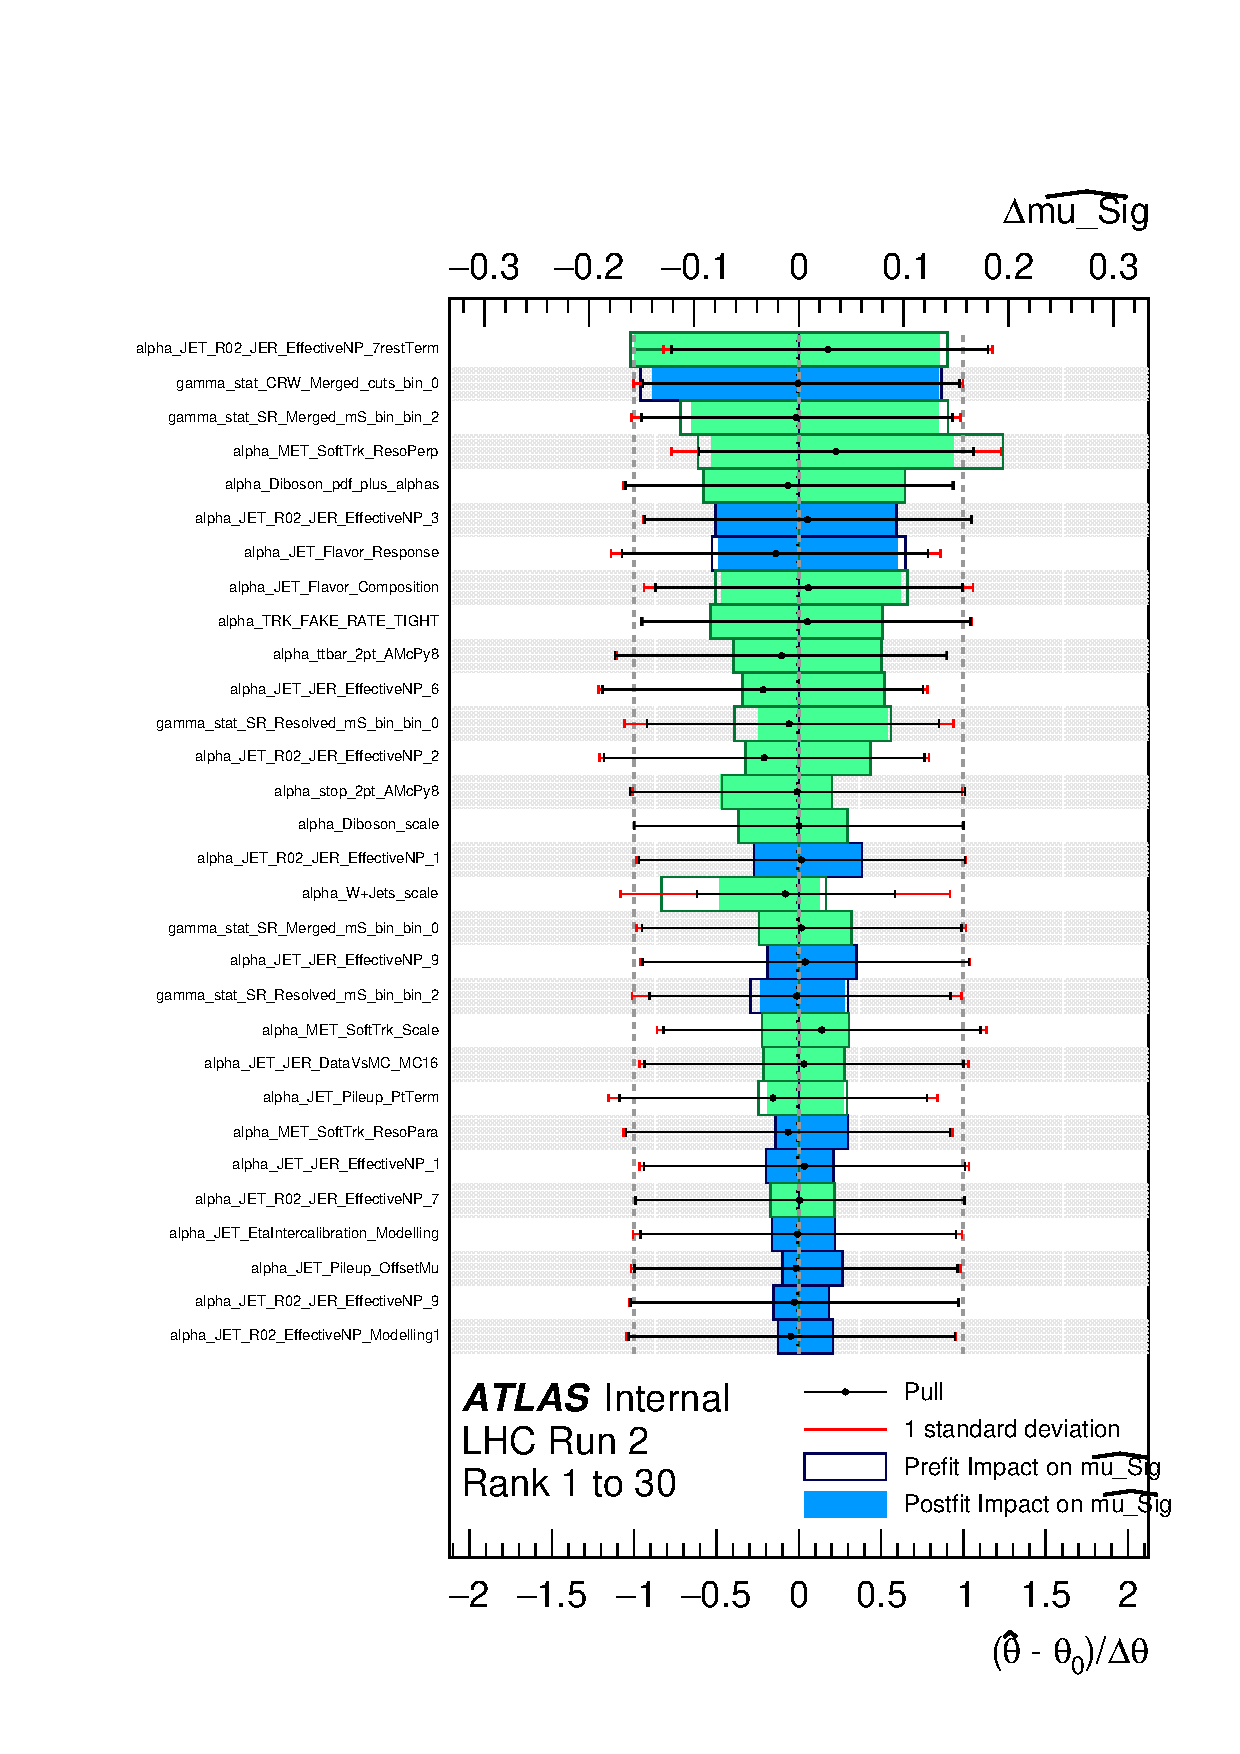
\includegraphics[width=0.9\textwidth]{Figures/8/ranking_mu_Sig_rank_0001_to_0030_zp2100_dm200_dh210_unblinded.pdf}
  \caption[Pre- and post-fit impacts for unblinded CRs (\ms, \mZp)=(210, 2100) GeV]{Leading 30 pre-and post-fit impacts on \(\mu_\text{Sig}\) for NPs associated with experimental and theoretical uncertainties in the signal+background fit at the sample signal point (\ms, \mZp)=(210, 2100) GeV. NPs are ranked from top to bottom in order of the size of their impact on \(\mu_\text{Sig}\). Blue (green) colouring of post-fit impacts indicates positive (negative) correlation with the signal strength. Post-fit values of the NPs (a.k.a. ``pulls") are also shown as black circles, where red (black) error bars show the size of the pre-fit (post-fit) uncertainty.}
  \label{fig:ranking_ms210}
\end{figure}

\subsection{Hypothesis Testing and Model Exclusion}

Hypothesis testing is performed following the method presented in Section \ref{sec:hypo_test} to determine the range of \ms and \mZp that can be confidently excluded by the search. The colour map in Figure \ref{fig:limits} shows the expected CL\(_s\) value evaluated over the range of \ms and \mZp considered in the search. Interpolated contours are drawn at CL\(_s=0.05\) for the expected (grey dashed) and observed (solid red) values, and the contained areas represent the expected and observed range of \ms and \mZp that are excluded by the search for the assumed DM mass and coupling choices.

\begin{figure}[h]
  \centering
  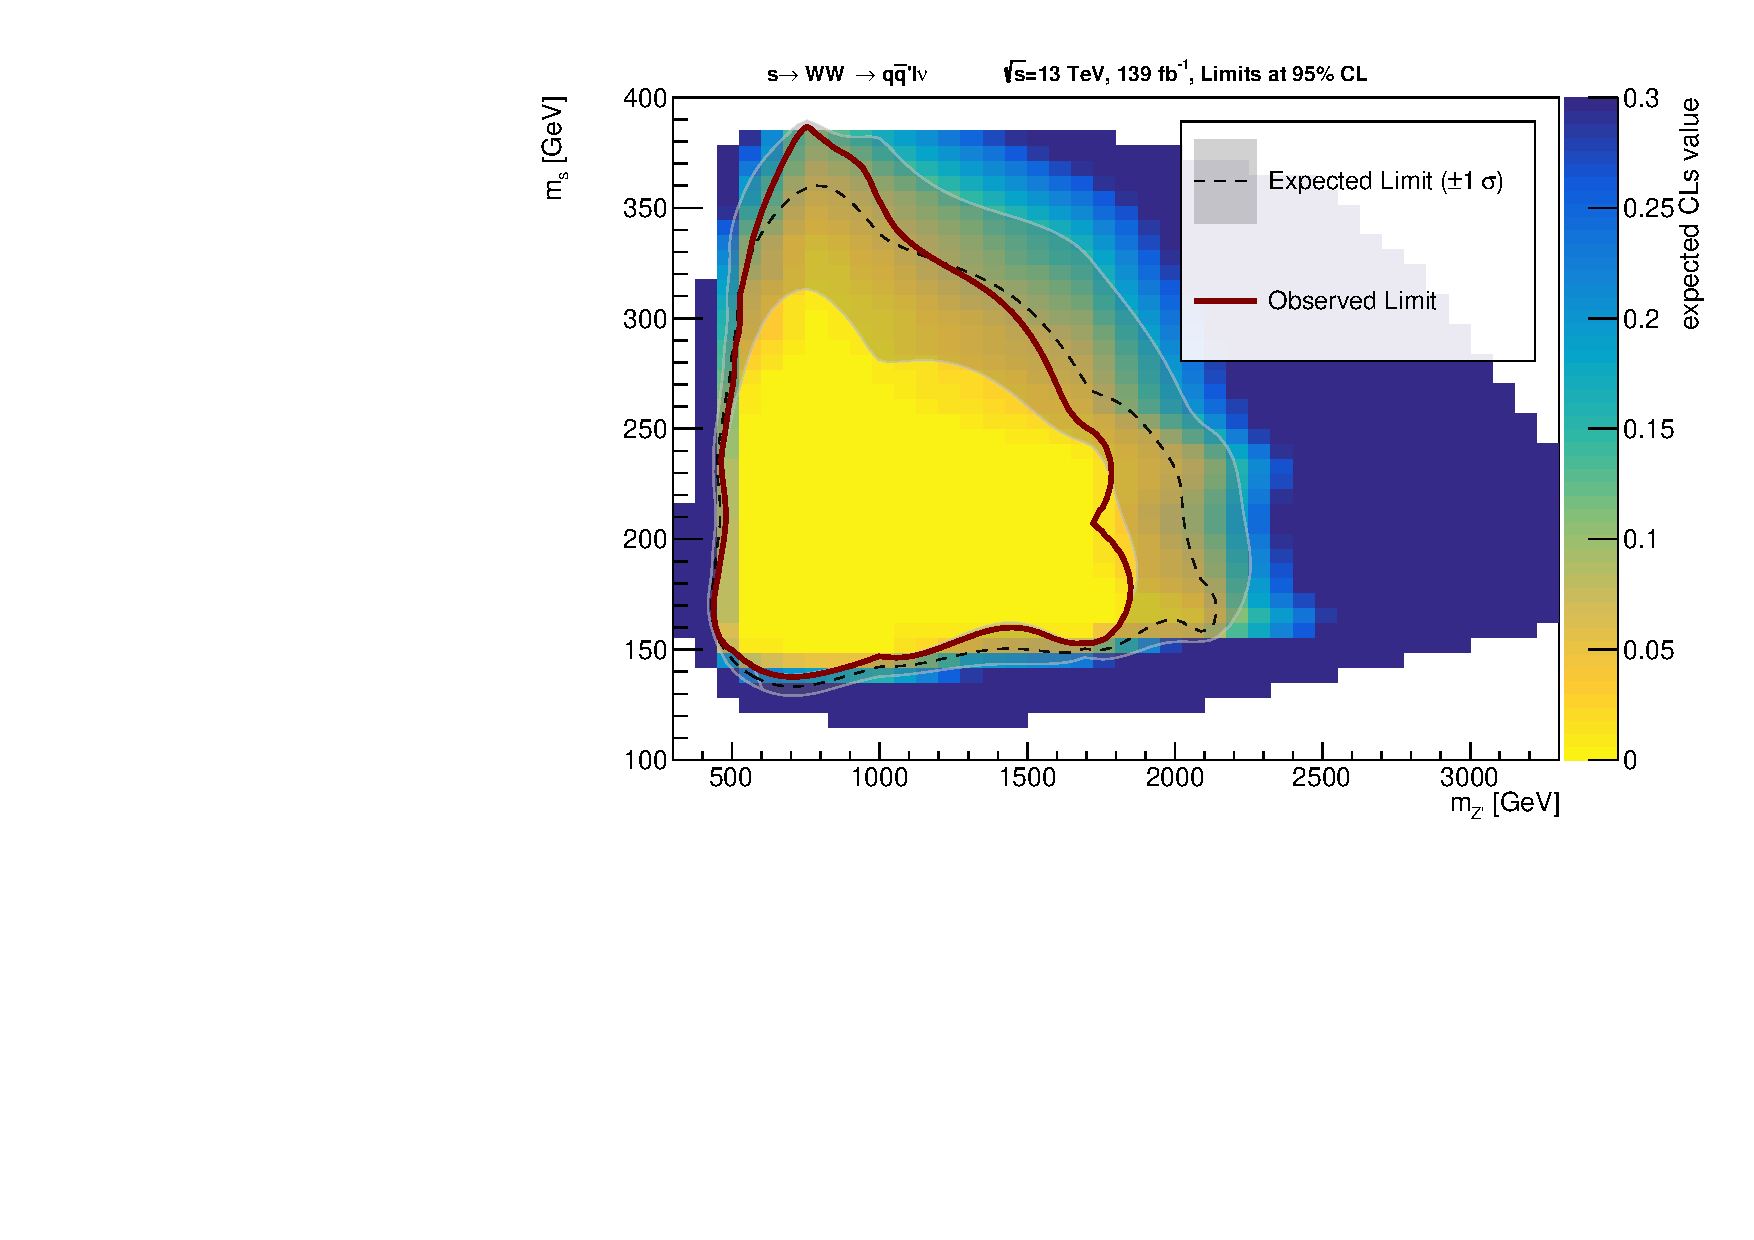
\includegraphics[width=0.8\textwidth]{Figures/8/unblinded_nosig.pdf}
  \caption[]{Expected (grey dashed with \(\pm1\sigma\) uncertainty band) and observed (solid red) range of \ms and \mZp in the DH model excluded by this search. All \ms and \mZp contained within the solid red line are excluded by the search for the choice of \(\mchi=200~\GeV\), \(\sin\theta=0.01\), \(\gchi=1.0\) and \(g_q=0.25\).}
  \label{fig:limits}
\end{figure}

Figure \ref{fig:limits_comparison} summarizes the excluded range of \ms and \mZp in the DH model - for the fixed choices of the DM mass, DH mixing angle and couplings presented at the beginning of this section - by this and all other searches presented in Section \ref{sec:dh_searches} which place constraints on the model by targeting various decay modes of the DH boson \(s\). This search (blue) extends the excluded range for on-shell \(WW\) decays (\(\ms>160~\GeV\)). By additionally probing off-shell \(WW\) decays in the range \(\ms<160\), this search largely closes the pre-existing gap in coverage (\(150~\GeV<\ms<160~\GeV\)) between searches in the \(s\rightarrow WW\) and \(s\rightarrow bb\) DH decay channels.

\begin{figure}[h]
  \centering
  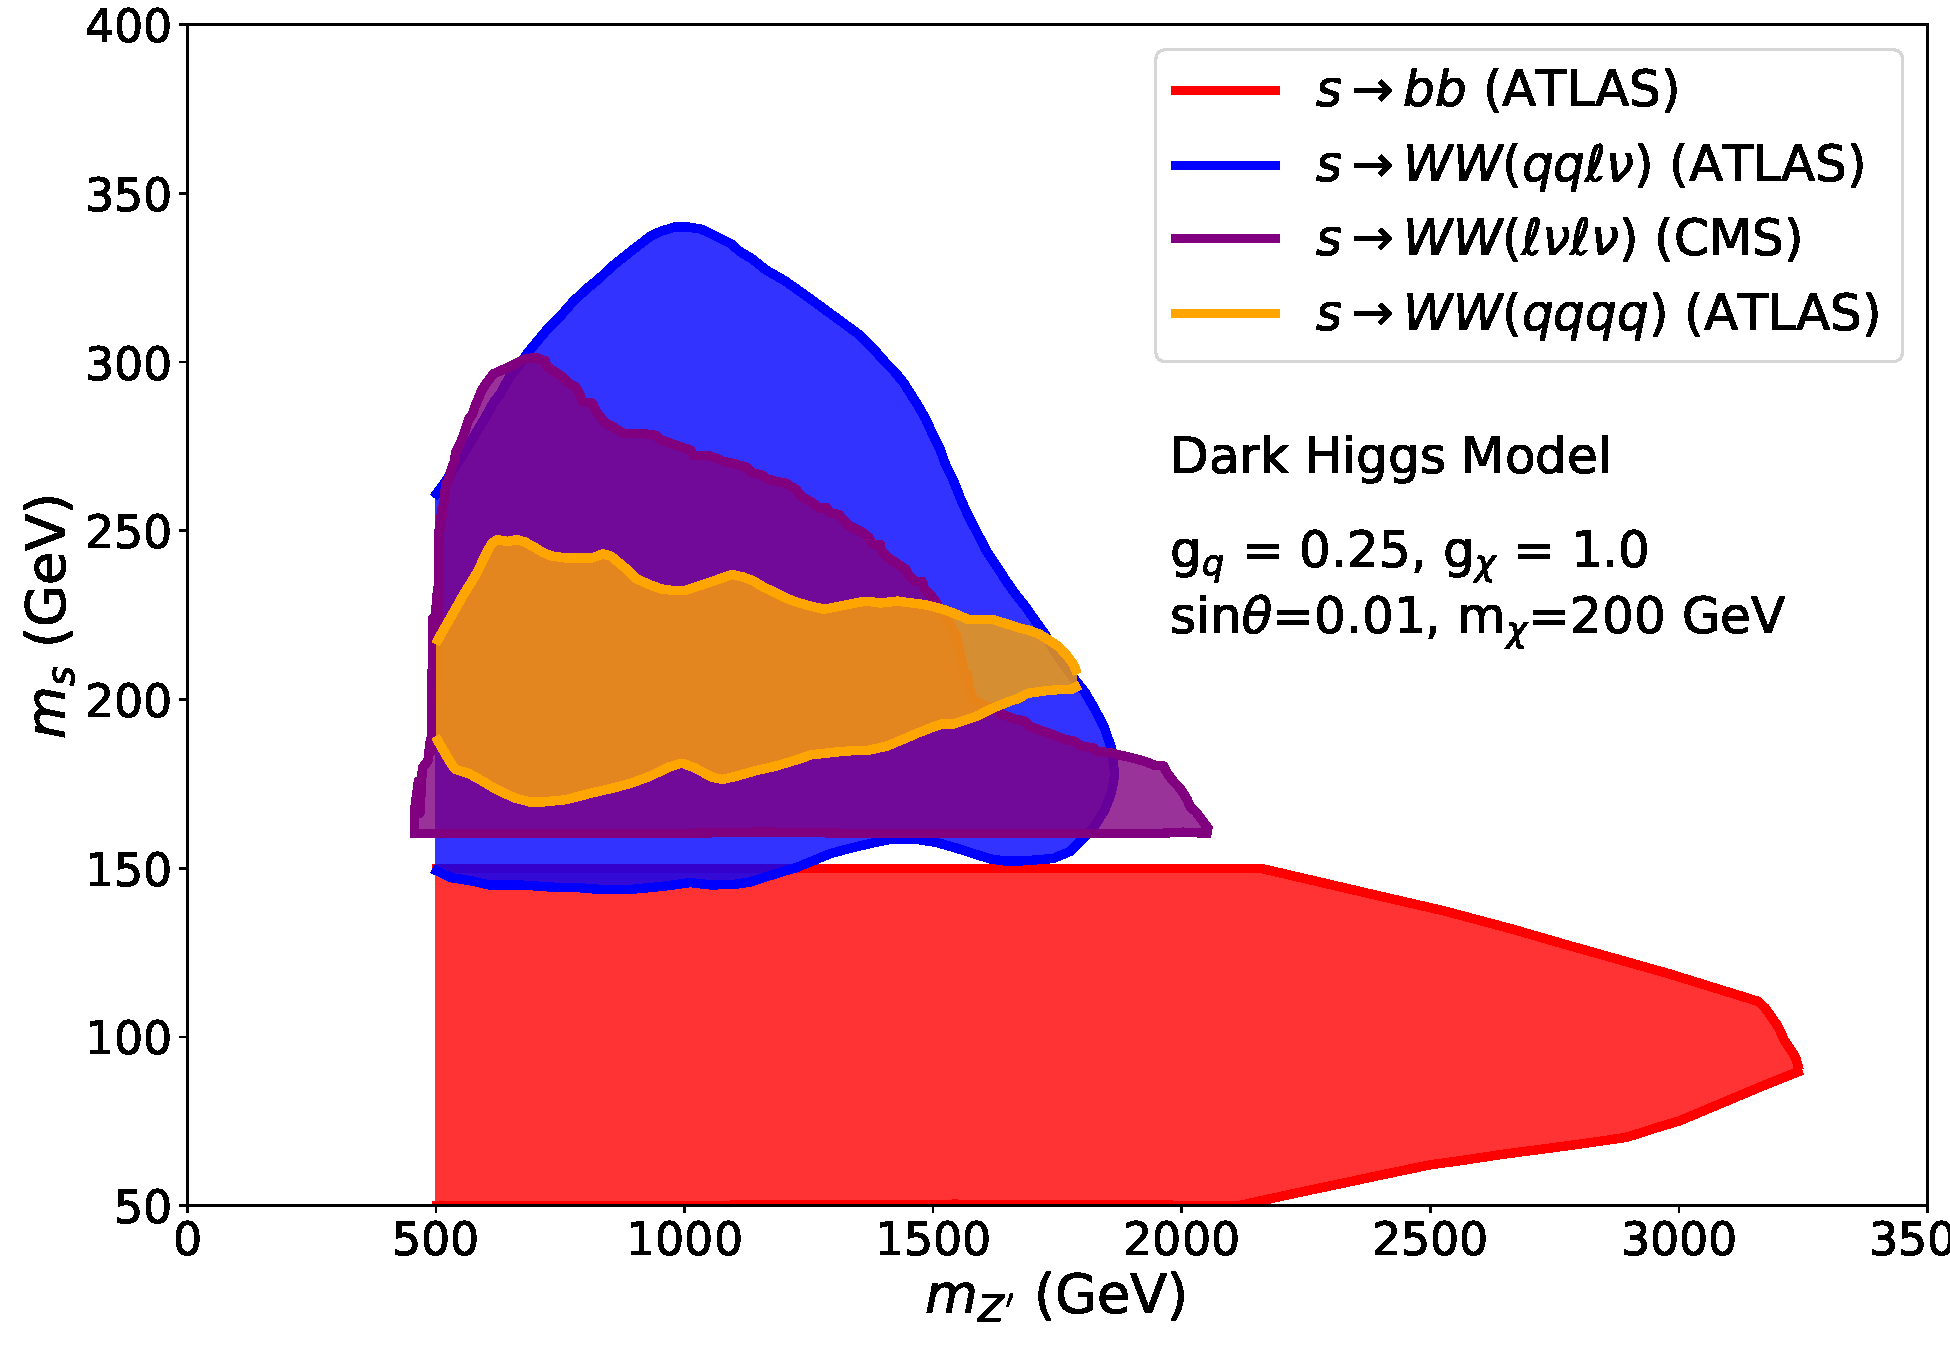
\includegraphics[width=0.8\textwidth]{Figures/8/combined_contour.pdf}
  \caption[]{Summary of \ms and \mZp parameters in the DH model excluded by all searches for the model by ATLAS and CMS. All values of \ms and \mZp contained within a coloured area are excluded. The range excluded by the search presented in this thesis is shown in blue.}
  \label{fig:limits_comparison}
\end{figure}


\subsection{Dependence of Sensitivity on Signal Strength}

Neglecting slight changes to the width of the \Zprime mediator, the production rate of the DH model would be expected to scale in proportion to \(g_q^2\) and \(\gchi^2\) \cite{griffiths_2008} if the values of the \(g_q\) and \(\gchi\) coupling strength parameters, respectively, are varied, since both correspond to a single annihilation (\(g_q\)) or decay (\gchi) vertex in the model (see Figure \ref{fig:Feynman_DH}). As noted in Section \ref{sec:dh_model_free_parameters}, upper bounds are placed on the coupling strength \(g_q\) between the \Zprime mediator and quarks in the DH model by dijet searches, which range from approximately 0.04 to 0.2 depending on the value of \mZp, and on the methods the assumptions involved in placing the constraints. However, the actual value of \gchi in the model is unknown, and is not currently constrained by dijet or other searches. 

Given the dependence of the production rate on the choices of \(g_q\) and \(\gchi\), a test was done following recommendations in Ref. \cite{boveia2016recommendations} to evaluate the impact of reducing the production rate of the DH process on the sensitivity of the search. Implicit in this test is a simplifying assumption that the modified values of \(g_q\) and \(\gchi\) associated with reducing \(\mu\) will result in the same distributions of kinematic variables as the benchmark choices, such that the predicted yields of the signal model in all regions and bins of the search scale linearly with \(\mu\). Figure \ref{fig:limits_vary_mu_sig} compares the range of \ms and \mZp excluded by the search with the value of a ``signal strength" parameter \(\mu\), which coherently scales the production rate of the DH signal process at all \ms and \mZp considered in the search. The search is able to exclude phase space in the \ms vs. \mZp plane for \(\mu\) down to 0.3, with the excluded range successively diminished as \(\mu\) is reduced.


